%!TEX program = xelatex
\documentclass{article}
\usepackage[
  a4paper,
  top=3cm,
  bottom=3cm,
  left=2cm,
  right=2cm
]{geometry}
\usepackage{ctex}
\usepackage{graphicx}
\usepackage{amsmath}
\usepackage{siunitx}
\usepackage{listingsutf8}

\title{悬链线理论}
\author{王勇 wangyong.seu@qq.com}
\begin{document}
\maketitle
\section{基本假设}
索由高强钢丝集束而成,相对抗弯刚度很小,其受力特点可以认为是完全柔性。
在自重和张力作用下分析其线形和力学参数时,基本假设如下:

\begin{itemize}
  \item
  索是理想柔性,既不能受压也不能受弯;
  \item
  索的材料符合胡克定律;
  \item
  索的横截面积在外荷载作用下的变化量十分微小,可忽略不计。
\end{itemize}

为了确定重力作用下索的线形,以弦左端点为原点、竖直向上为Y轴正方向建立右手直角坐标系。
则索受到的重力沿Y轴负向。
假设单位长度索的质量恒定,且不随张力变化。

\begin{figure}
  \centering
  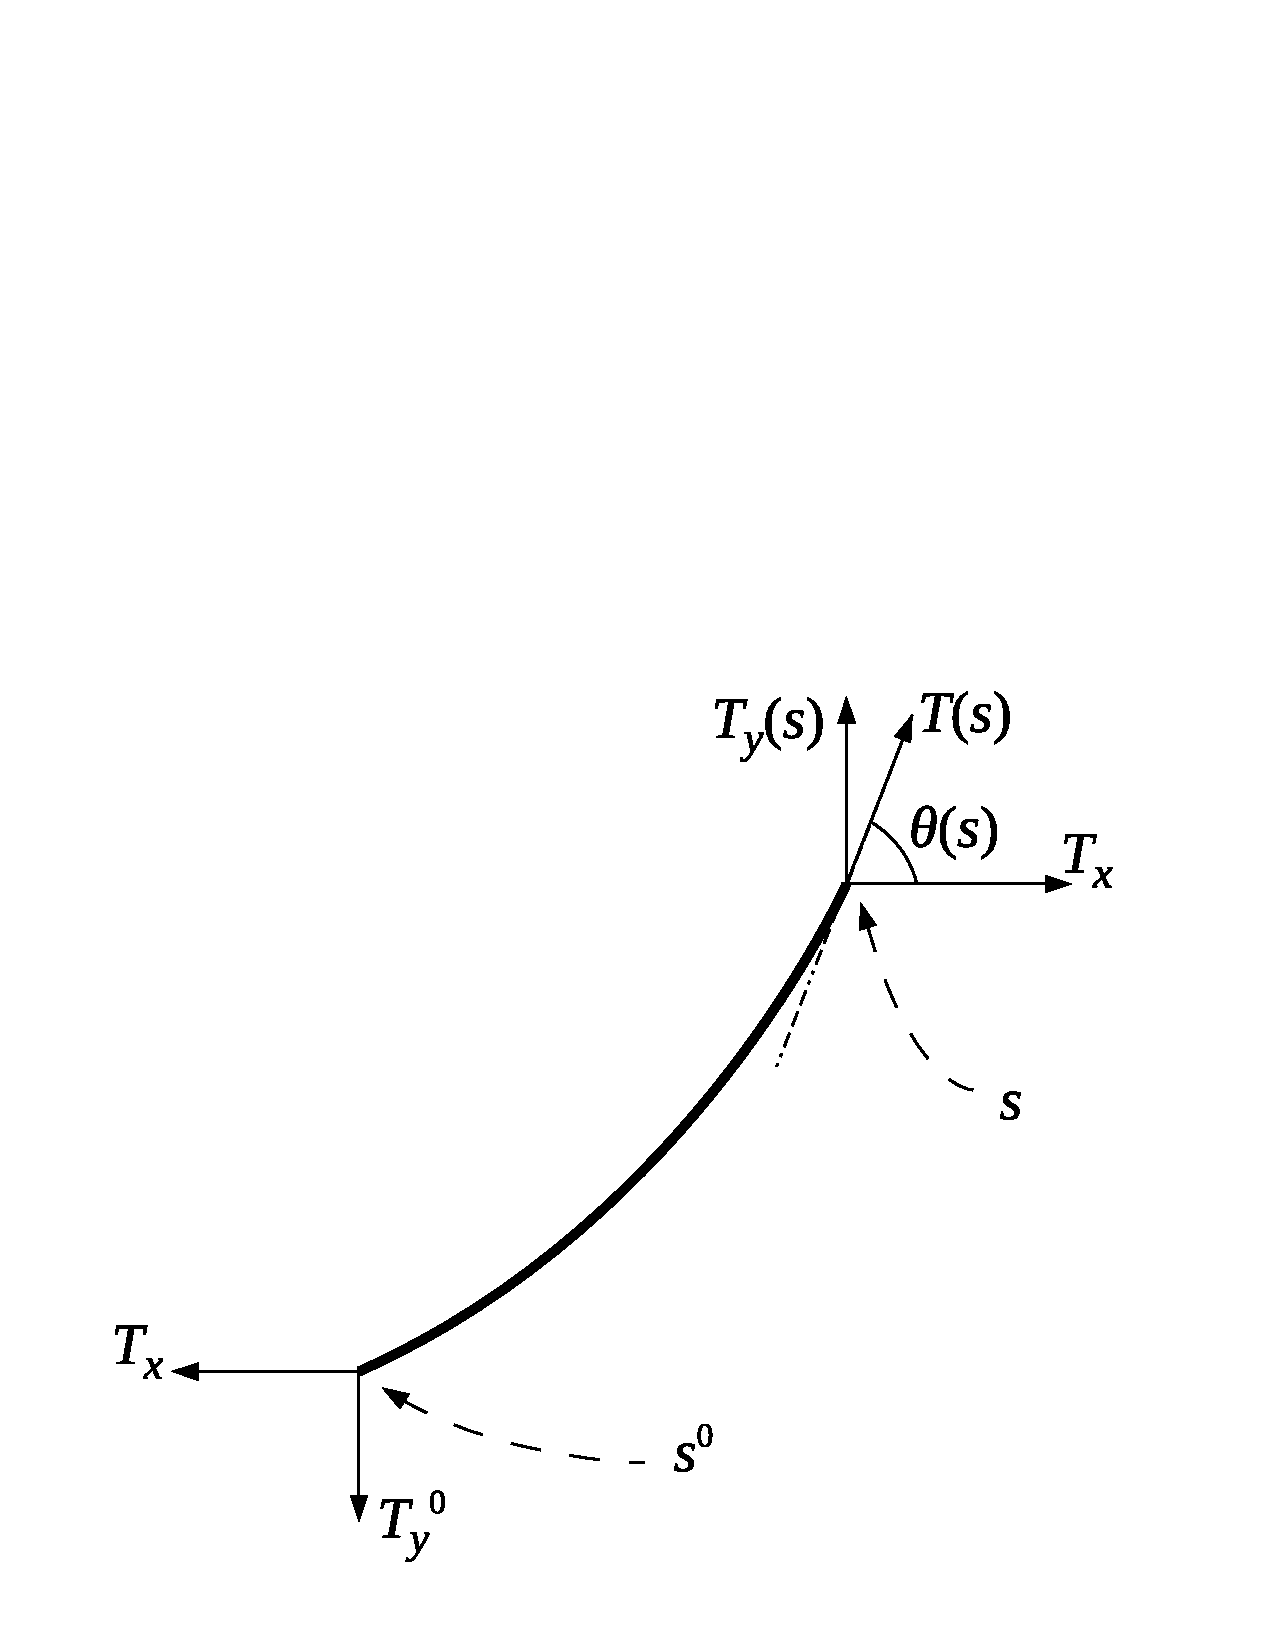
\includegraphics[width=0.6\textwidth]{./fig/catenary_diagram.pdf}
  \label{fig:catenary}
  \caption{索段计算示意图}
\end{figure}

\section{符号约定}
\begin{description}
  \item[$s$]
  从索左端点(坐标系原点)开始计算的索长度;
  \item[$\mu$]
  单位长度索的质量(假设是恒定的);
  \item[$T(s)$]
  索长度为$s$处的索张力(根据柔性索假设,张力沿索的切线方向);
  \item[$T_y(s)$]
  索长度为$s$处的索张力的$Y$向分量;
  \item[$T_x$]
  张力的$X$向分量(任取索段进行受力分析,由$X$向平衡方程可知$T_x$沿索长是均匀的);
  \item[$\theta(s)$]
  索切向量与$X$轴正向的夹角。
\end{description}

\section{索曲线求解}
索段竖向的平衡方程为:
\begin{gather}
  T_y(s) = g \int_{s^0}^{s} \mu \mathrm{d}s + T_y^0 \notag \\
  T_x \tan(\theta(s)) = g \mu \int_{s^0}^{s} \mathrm{d}s + T_y^0 \notag \\
  T_x \frac{\mathrm{d} y}{\mathrm{d} x} = g \mu \int_{s^0}^{s} \sqrt{1+\left(\frac{\mathrm{d} y}{\mathrm{d} x}\right)^2} \mathrm{d}x + T_y^0 \notag \\
  \frac{\mathrm{d}^2 y}{\mathrm{d} x^2} = \frac{g \mu}{T_x} \sqrt{1+\left(\frac{\mathrm{d} y}{\mathrm{d} x}\right)^2}
\end{gather}
此二阶微分方程的解析解为:
\begin{equation}
  y = \frac{T_x}{g \mu} \cosh \left( \frac{g \mu}{T_x} + c_1 \right)+c_2
\end{equation}
式中,$c_1$和$c_2$为由边界条件确定的积分常量。代入边界条件:$x=0,y=0;x=L,y=C$得:

\begin{equation}
  \left \{
    \begin{split}
      & \beta = \frac{g \mu L}{2 T_x}\\
      & c_1 = \sinh^{-1}\left(\frac{\beta C / L}{\sinh \beta}\right)\\
      & c_2 = -\frac{T_x}{g \mu} \cosh(c_1)
    \end{split}
  \right.
\end{equation}

悬链线索的形状长度$S$和无应力长度$S_0$分别为:
\begin{equation}
  S = \frac{T_x}{g\mu}\left[\sinh\left(\frac{g \mu L}{T_x}+c_1\right)+\sinh(c_1)\right]
\end{equation}

\begin{equation}
\begin{split}
  S_0 &= S-\Delta S \\
      &= S - \frac{T_x}{EA g \mu }\left[ \frac{1}{2} g \mu L + \frac{1}{8} T_x \left( e^{2(c_1+2\beta)} - e^{-2(c_1-2\beta)} -e^{2c_1} + e^{-2c_1} \right) \right]
\end{split}
\end{equation}
\section{算例}
问题描述:一根跨度为$L=\SI{888}{m}$,右侧支座比左侧支座低\SI{80}{m},跨中矢高$f=\SI{100}{m}$,每延米重$g \mu=\SI{60}{kN/m}$。
索的弹性模量$E=\SI{2E5}{MPa}$,面积$A=\SI{0.6}{m^2}$。
假设在外荷载作用下两支座的间距及高差保持不变。
试求如下参数:索的水平力$T_x$,索的无应力长度$S_0$及索在受荷载作用下的形状长度$S$。

解题思路:单缆在自重和张力作用下,其线形为悬链线,故可采用悬链线经典公式来进行求解。
采用直接建模的方式,单缆采用LINK1单元模拟,单元水平长度为\SI{1}{m}。
分析时,首先假定水平力大小,根据悬链线方程求解节点坐标,由此建立节点和单元,并分析单缆在自重作用下的内力和线形。
如果求解获得的水平力与假定水平力之间的误差较大或者单缆变形较大,则返回重新计算,直至满足误差要求。

\lstinputlisting{./fea/apdl.mac}

\begin{figure}[!h]
  \centering
  \label{fig:result}
  \includegraphics[width=\textwidth]{fig/disp.pdf}
  \caption{单缆变形图}
\end{figure}

结果分析,如图\ref{fig:result}所示,单缆在自重作用下的最大竖向位移为\SI{3.142}{mm},相比于跨径,改变形足够小,认为已满足精度要求。
此时求得的单缆力学参数如下:
单缆水平力$T_x = \SI{99549.776}{kN}$,受荷后曲线长度为$S=\SI{902.1906}{m}$,单缆伸长量$\Delta S=\SI{0.7606}{m}$,无应力长度为$S_0 = \SI{901.4299}{m}$。
\end{document}
